\documentclass[letterpaper,10pt,twocolumn]{article}

\usepackage{footmisc}
%\usepackage[T1]{fontenc}
%\usepackage{fontspec}
%\setmainfont{Times New Roman}
\usepackage{times}
\usepackage{xcolor}
\usepackage{xspace}
\usepackage{type1cm}
\usepackage{boxedminipage}
\usepackage{pifont}
\usepackage{pseudocode}
\usepackage{multirow}
\usepackage{tabularx}
\usepackage{caption}
\usepackage{amsmath}
\DeclareCaptionType{copyrightbox}
\usepackage{subcaption}

\definecolor{MyDarkBlue}{rgb}{0,0.08,0.45}
\usepackage[pdftex]{hyperref}
\hypersetup{
  colorlinks,%
  citecolor=MyDarkBlue,%
  filecolor=MyDarkBlue,%
  linkcolor=MyDarkBlue,%
  urlcolor=MyDarkBlue
}
\usepackage{fixltx2e}
\usepackage{textgreek}
\usepackage[sort]{cite}

% ----------------- Macros: ---------------------
\newcommand{\projectname}{{STS}}
\newcommand{\projectmeaning}{SDN Troubleshooting System}

\newcommand{\tester}{mock network}

\newcommand{\simulator}{retrospective causal inference}
\newcommand{\Simulator}{Retrospective causal inference}
\newcommand{\SIMULATOR}{Retrospective Causal Inference}
\newcommand{\tbd}[1]{{\bf [[TBD: {#1}]]}}
\newcommand{\ie}{{\it i.e.}}
\newcommand{\eg}{{\it e.g.}}
\newcommand{\cf}{{\it cf.}}
\newcommand{\etc}{{\it etc.}}
\newcommand{\viz}{{\it viz.}}
\newcommand{\apriori}{{\it a priori}}
\newcommand{\eat}[1]{}

% ---------------- Notes: -----------------------
\newcommand{\num}[1]{{\color{red}\bf {#1}}}

%\newcommand{\teemu}[1]{{\color{ForestGreen}\bf TK: {#1}}}
%\newcommand{\andi}[1]{{\color{blue}\bf AW: {#1}}}
%\newcommand{\sam}[1]{{\color{orange}\bf SW: {#1}}}
%\newcommand{\colin}[1]{{\color{red}\bf CS: {#1}}}
%\newcommand{\scott}[1]{{\color{purple}\bf SS: {#1}}}
\newcommand{\barath}[1]{{\color{red}\bf BR: {#1}}}

\newcommand{\teemu}[1]{}
\newcommand{\andi}[1]{}
\newcommand{\sam}[1]{}
\newcommand{\colin}[1]{}
\newcommand{\scott}[1]{}
%\newcommand{\barath}[1]{}

% ------------ Macros for generating graphical event sequences: -----------
\usepackage{tikz}
% External event. Takes label as parameter.
\newcommand{\external}[1]{
\tikz[baseline=-0.5ex]\draw[black,fill=white] (0,0)
node[rounded corners,fill=red!60,draw,inner sep=0pt,minimum size=0.4cm] {$e_{#1}$};}%
% Internal event. Takes label as parameter.
\newcommand{\internal}[1]{
\tikz[baseline=-0.5ex]\draw[black,fill=white] (0,0)
node[rounded corners,fill=green!80,draw,inner sep=0pt,minimum size=0.4cm] {$i_{#1}$};}%

\makeatletter
% Functional foreach construct
% #1 - Function to call on each comma-separated item in #3
% #2 - Parameter to pass to function in #1 as first parameter
% #3 - Comma-separated list of items to pass as second parameter to function #1
\def\foreach#1#2#3{%
  \@test@foreach{#1}{#2}#3,\@end@token%
}

% Internal helper function - Eats one input
\def\@swallow#1{}

% Internal helper function - Checks the next character after #1 and #2 and
% continues loop iteration if \@end@token is not found
\def\@test@foreach#1#2{%
  \@ifnextchar\@end@token%
    {\@swallow}%
    {\@foreach{#1}{#2}}%
}

% Internal helper function - Calls #1{#2}{#3} and recurses
% The magic of splitting the third parameter occurs in the pattern matching of the \def
\def\@foreach#1#2#3,#4\@end@token{%
  #1{#2}{#3}%
  \@test@foreach{#1}{#2}#4\@end@token%
}

\makeatother

% Helper method, prepends a rightarrow before a node, throws away first
% argument
% TODO(cs): figure out how to make this a private method.
\def\connecthelper#1#2{#2$\mathtt{\rightarrow\mkern-6mu}$}
% Prepend a rightarrow before a node
\def\connect#1{\connecthelper{}{#1}}

% Chain together a list of nodes. Takes two parameters:
% #1: a comma-delimited list of the of everything in the list *except* the
% last element.
% #2: the *tail* of the chain
% TODO(cs): figure out how to delimit the first comma so that tail doesn't
% need to be specified separately.
\def\chain#1#2{\foreach{\connecthelper}{}{#1}$\mathtt{\;\cdot\!\!\cdot\!\!\cdot\mkern-5mu}$#2}

% Chain together a list of nodes, with two tails, separated by dots. Takes three parameters:
% #1: a comma-delimited list of the of everything in the list *except* the
% last element.
% #2: the first tail of the chain
% #2: the second tail of the chain
\def\doublechain#1#2#3{\chain{#1}{#2}$\mathtt{\rightarrow\mkern-6mu\cdot\!\!\cdot\!\!\cdot\mkern-4mu}$#3}

\def\eventlist#1#2{$\mathtt{\text{#1}\!\cdot\!\!\cdot\!\!\cdot\mkern-8mu\text{#2}}$}

% -------------- Delta-debugging symbols: -----------
\newcommand{\PASS}{\text{\ding{52}}\xspace}
\newcommand{\DFAIL}{\text{\ding{56}}\xspace}
\newcommand{\cpass}{{T_{\scriptscriptstyle \PASS}}}
\newcommand{\cfail}{{T_{\scriptscriptstyle \DFAIL}}}
\newcommand{\dpass}{{T'_{\scriptscriptstyle \PASS}}}
\newcommand{\dfail}{{T'_{\scriptscriptstyle \DFAIL}}}
\newcommand{\done}{{T_{\scriptscriptstyle 1}}}
\newcommand{\dtwo}{{T_{\scriptscriptstyle 2}}}
\newcommand{\test}{\textit{test}\xspace}
\newcommand{\ddmin}{\textit{ddmin}\xspace}

\sloppy

\title{Minimizing Test Cases For Distributed Systems}
\author{Colin Scott \\
Qualifying Exam Proposal \\
UC Berkeley Department of Computer Science \\
October 30th 2014
}
\date{}

% Prompt:

% Your summary should survey that area and describe open and interesting
% research problems.

% Describe why you chose these problems and indicate what direction your
% research may take in the future.

% It will include a summary of research to date and plans for future work (or
% at least the next stage thereof).

\begin{document}
   \maketitle
   \thispagestyle{empty}

\abstract{{\it The predominant technique for troubleshooting bugs in software-defined networks,
log analysis, is tedious and error-prone. We argue that a more principled
approach should be built around identifying inconsistencies between lower-level
network configuration and higher-level policies dictated by control
applications. Towards this end we present
cross-layer correspondence checking, a mechanism to automatically detect and
isolate inconsistencies due to bugs in the SDN platform. In
eventually-consistent systems such as SDN however,
transient inconsistencies between policy and configuration are inevitable.
We therefore augment correspondence checking with \simulator{} to help troubleshooters
distinguish pernicious persistent from harmless ephemeral inconsistencies. We
show that these techniques combine to help troubleshooters ``see through the fog'' of
diagnostic information.
}}

\section{Introduction}
\label{sec:intro}
The SDN platform's $raison\text{ }d'\hat{e}tre$ is to 
hide complexity from control applications. Modern controllers perform
replication, resource arbitration, failure recovery, and network 
virtualization on the control application's behalf. 

Despite the abstractions provided by the SDN programming model,
software-defined networks are no less complex than traditional networks. The architectural goal of SDN is
simply to push complexity from the control application onto the underlying platform.

SDN control platforms are prone to bugs as a result of their complexity. Bugs in the
platform present an architectural tension: troubleshooting requires
access to precisely the same details hidden by the platform's abstractions.
When an application developer 
encounters erratic behavior in the network, they must trace their
policy specification through multiple layers of abstraction
preceding changes in the physical network: virtualization logic,
distribution logic, and network devices. The error's root cause
may manifest in any of these layers, not just the control application.

As it stands, the SDN platform provides meager support for troubleshooting.
The predominant troubleshooting method is log analysis: manually
specifying log statements at relevent points throughout the system,
collecting, gathering, and ordering distributed log files, and analyzing the
results {\it post-hoc} when a error is encountered in production. Besides its
apparent tediousness, this approach is lacking in several ways: logs events
are enormous in number, impossible to aggregate into a single serial
execution of the system, and often at the wrong level of granularity to be of
use. \colin{</ why it's hard>}

Recent work has contributed much-needed improvements to this state of affairs. 
NICE applies concolic execution and model checking to SDN control
applications, thereby automating testing and catching bugs before
they are deployed~\cite{nice}. Aneater~\cite{anteater} and HSA~\cite{hsa}
introduce mechanisms for checking static invariants in the dataplane.
Nevertheless, no troubleshooting mechanism exists yet for the SDN platform itself.

New operating system abstractions face an arduous path towards adoption
without sound troubleshooting mechanisms. Analogously, the success of the
SDN programming model depends heavily on the utility of its troubleshooting
paradigm. Our goal in this paper is to work towards a useful
troubleshooting mechanism for the SDN platform. \colin{</ why it's important>}

We observe that in eventually-consistent systems such as sofware-defined networks,
transient inconsistencies are an inevitable property of the system.
Consequently, the process of troubleshooting errors essentially boils down to
identifying relevant events amongst a clamor of inconsistencies and diagnostic
information.

We present two mechanisms designed to make it easier for operators and
developers to ``see through the noise'' of diagnostic information. The first,
cross-layer correspondence checking, leverages the structure of the SDN
architecture to enable a general and verifiable notion of platform
correctness. Correspondence checking allows troubleshooters to isolate the cause of 
an inconsistency to a particular layer without needing to define invariants or
instrument third-party code. Our second
mechanism, simulated replay analysis, allows troubleshooters 
to differentiating ephemeral from persisent inconsistencies by steering the
execution of the system forward and backward in time, filtering out extraneous
external events, and inducing uncommon events such as failures. \colin{</ what we did>}

The rest of this paper is organized as follows. In \S\ref{sec:overview},
we present an overview of the SDN stack and its failure modes.
In \S\ref{sec:approach} we present correspondence checking and simulated
replay analysis in detail. In \S\ref{sec:evaluation} we present
two use-cases of our techniques, as well as a preliminary evaluation
of their runtime. Finally, in \S\ref{sec:related_work} we discuss related work,
and in \S\ref{sec:conclusion} we conclude.


\section{Problem Definition}
\label{sec:formalism}
We represent the forwarding state of the network
at a particular time as a configuration $C$.
An invariant is a predicate $P$ over forwarding state (a safety
condition). We say that forwarding
state $C$ violates an invariant if $P(C)$ does not
hold, also denoted as $\overline{P}(C)$.

Log $L$ consists of external events $E_L$ and observed internal events $I_L$,
along with a timing $T_L$ of the observed events.
We assume that all changes to forwarding state can be inferred
from internal events (\eg~OpenFlow message sends), so
that at all times we have knowledge of the relevant forwarding state.
Therefore we can determine from $L$ whether $P$ failed to hold at any point.
% It might make the notation more concise if we just include the sequence of
% forwarding configurations as part of L. We have access to this information
% in practice, since we're driving the fuzzing.

A replay of a log means replaying the external events along with a particular timing (or interleaving) $T$.
We denote this by $replay(E_L,T)$.
The output of $replay$ is a sequence of forwarding state configurations
$C_1,C_2,\dots,C_n$.
We say that a replay reproduces an invariant violation if
$\exists_{C_i \in replay(E,T)}\:s.t.\:\overline{P}(C_i)$.
In the ideal case $replay(E_L,T_L)$ reproduces the orignal invariant violation
asociated with $L$ (as long as there is no nondeterminism). \\

\noindent~Troubleshooting process:

\begin{outline}
\1 Start with log $L$ where $P$ did not hold at some point. Could be operational or fuzzed log.

\1 Definition: an MCS is a subsequence $E_M$ of $E_L$ and a timing $T_M$ such
that $replay(E_M,T_M)$ reproduces the invariant violation, but for all proper
subsets $E_L$ of $E_M$
there is no timing $T$ s.t. $replay(E_L,T)$ reproduces the violation.

\1 Assumption 1: naturally occurring external logs $E_L$ are large.

\1 Assumption 2: the MCS of most natural logs resulting in violations are much smaller than the original log.  That is, bugs are causally sparse.
\end{outline}

\noindent~Technical challenge: Find approximations to MCSs.

\begin{outline}
\1 Dumb approach: explore all timings $T$ for each subset $E$.

\1 Slightly smarter approach: use delta debugging, causality, and equivalence to limit set of timings $T$ you need to look at.
\end{outline}


\section{Related Work}
\label{sec:related_work}
%-- Program Slicing --

The delta debugging algorithm~\cite{Zeller:2002:SIF:506201.506206} seeks to solve
a problem that is exactly analogous to ours on a single machine: given input that causes a test case
to fail, what is the minimum subset of the input that still produces the failure?
We apply the same reasoning to a distributed system.

%-- Deterministic Replay (OFRewind) --

Deterministic replay techniques such as OFRewind~\cite{ofrewind}
are designed to allow developers to interactively prune
the inputs that lead up to errant behavior. We present an algorithm that
automates this process.

%-- Model checking (NICE): --

NICE~\cite{nice} combines model checking with concolic execution
to enumerate all possible code paths taken by control software (NOX)
and identify concrete inputs (\eg{} control message orderings) that cause
the network to enter invalid configurations. Unlike NICE, by analyzing
bugs {\em post-hoc} from live runs of the system our approach applies
to large software systems without suffering from state explosion.

%-- Invariant Checking? --

\eat{
Invariant checking tools such as Anteater~\cite{anteater} and HSA~\cite{hsa}
detect problems in the dataplane. We leverage invariant checking tools
to distinguish inputs that are necessary for reproducing a given invariant violation.
}

%-- Root cause analysis? --

Root cause analysis techniques~\cite{577079} seek to identify the minimum set of failed
components (\eg{} link failures) needed to explain a collection of alarms. Rather than
focusing on individual component failures, we seek to minimize inputs that affect the behavior
of the overall distributed system.

%-- Distributed Systems debuggers --

Pip~\cite{pip} is a framework for instrumenting general-purpose distributed systems
with code to record, display, and check invariants on causal paths throughout
live executions. \Simulator{} observes the causal behavior of the
distributed system in a simulated environment, enabling us to iteratively prune extraneous input events.

%-- Simulators? --
%
%Several other network simulators exist for testing SDN controllers. Mininet is a
%platform for emulating OpenFlow switches and hosts within a single
% VM~\cite{Lantz:2010:NLR:1868447.1868466}. The ns-series of network simulators
%provides a general framework for testing new protocols, topologies,
%and traffic mixes~\cite{ns3}. We found that these existing simulators did
%not provide sufficient support for the corner-cases situations which are the
%focus of our work, such as failures and VM migration.

%-- Distributed Systems --
%
%Many of our ideas originate from the literature on troubleshooting general
%distributed systems. WiDS checker introduced the notion of recording
%production executions to be later replayed and verified in a controlled simulation.
% Finally, end-to-end tracing
%frameworks such as X-Trace~\cite{Fonseca:2007:XPN:1973430.1973450} and
%Pinpoint~\cite{Chen02pinpoint:problem} provide a framework for tracing requests throughout
%a distributed system in order to infer correctness errors between layers and
%across components. Our work solves a more constrained problem; we leverage
%the structure of the SDN stack to enable a simple notion of platform
%correctness. In addition, these systems assume that invariants should hold at
%all times; we observe that in an eventually-consistent system such as SDN,
%transient policy-violations are inevitable. We built \simulator{} to help troubleshooters
%differentiate ephemeral from persistent errors.

% If we manage to run multiple applications by Monday, we should cite papers
% on consistency and cross-layer debugging:
%X-Trace~\cite{xtrace}
% Vector Clocks
% Onix
% Virtualization definitely won't happen by Monday. But, papers include
% Martin's presto '10 paper 'Virtualizaing the Network Forwarding Plane'



\section{Past Work}
\label{sec:past_work}
In this section we present heuristics we previously developed and applied to one kind of
distributed system: software-defined networking (SDN) control software. Here, we begin by briefly describing the behavior of SDN
control software.

\noindent {\bf Overview of SDN Control Software.} Network operating systems, the key component of SDN software
infrastructure, consist of control software running on a replicated set of
servers, each running a controller instance. Controllers coordinate between
themselves, and receive input events (\eg~link failure notifications) and
statistics from switches (either physical or virtual), policy
changes via a management interface, and possibly dataplane packets.
In response, the
controllers issue forwarding instructions to switches. All input
events are asynchronous, and individual controllers may fail at any
time. The controllers either communicate
with each other over the dataplane network, or use a separate dedicated
network, and may become partitioned.

%\subsection{Bugs, QA Testing, and Troubleshooting}
The goal of the network control plane is to configure the switch forwarding entries so as to
enforce one or more invariants, such as connectivity (\ie~ensuring that a
route exists between every endpoint pair), isolation and access control
(\ie~various limitations on
connectivity), and virtualization (\ie~ensuring that packets are handled
in a manner consistent with the specified virtual network).
A bug causes an invariant to be violated. Invariants can be
violated because the system was improperly configured
%A bug causes an invariant to be violated. Bugs can occur in the
%configuration management system, \eg~OpenStack~\cite{quantum}
(\eg~the management system~\cite{quantum} or a human improperly specified their goals), or
because there is a bug within the SDN control plane itself. In this paper we focus on troubleshooting bugs in the
SDN control plane after it has been given a valid policy configuration.\footnote{This does
not preclude us from troubleshooting misspecified policies
so long as test
invariants~\cite{hsa} are specified separately.}

\noindent {\bf Heuristics for Accounting for Interleavings.} To reproduce an invariant
violation found in an execution of SDN control software,
we need to inject each input event \external{} only after all other
events, including internal events,
that precede it in the
happens-before relation~\cite{Lamport:1978:TCO:359545.359563} from the
original execution ($\{i \mid i \rightarrow\!\!\text{\external{}}\}$) have
occurred~\cite{tel2000introduction}.

The internal events we consider are
(a) message delivery events, either between controllers (\eg~database
synchronization messages) or
between controllers and switches (\eg~OpenFlow messages), and (b) state transitions
within controllers (\eg~a backup node deciding to become master).
Our replay orchestrator obtains visibility into (a) by interposing on all messages within the test
environment (described in detail in~\cite{sts2014}).
It optionally obtains partial visibility into (b) by instrumenting controller
software with a simple interposition layer (described in~\cite{sts2014}).

%From the perpsective
%By virtue of managing inputs and message deliveries from a central location, we are
%able to totally-order the event trace $\tau_L$.
%We thereby augment the log $(E_L, T_L)$ with a schedule
%$\tau_L\!=\!e_1\!\rightarrow\!i_1\!\rightarrow\!\dots\!e_2\!\rightarrow\!\dots$, where
%each $i$ is an internal event observed in the original run.

\colin{Add back in (reword) if we have space:}
%Note that we do not control the occurrence of internal events, and therefore do
%not attempt to minimize them. Crucially though, we need to ensure that the ordering
%of input and internal events during
%$replay()$ of each subsequence is consistent with the happens-before relation,
%so that we can report invariant violations
%(minimization opportunities) to delta debugging as often as possible.
%To meet this requirement our test orchestrator may use its interposition on
%messages to reorder or drop messages as necessary during replay.
%The final MCS produced by our system therefore includes a schedule
%$\tau_S\!=\!e_1\!\rightarrow\!i_1'\!\rightarrow\!\dots\!e_2\!\rightarrow\!\dots$
%reflecting how the minimal subsequence of inputs should be interleaved
%with internal events in order to reproduce the invariant violation. This
%schedule supersedes the timings $T$ described in \S\ref{sec:formalism}.

%\subsection{Preserving Causality}

\begin{table}[tb]
\centering
\footnotesize
\begin{tabular}{|l|l|}
\hline
{\bf Internal Message} & {\bf Masked Values} \\
\hline
\hline
OpenFlow messages & xac id, cookie, buffer id, stats \\
% port numbers?
\hline
packet\_out/in payload & all values except src, dst, data \\
\hline
Log statements & varargs parameters to printf \\
\hline
\end{tabular}
\caption{Internal messages and their masked values. %The masks serve to
%define equivalence classes.
}
\label{tab:fingerprints}
\vspace{-0.6cm}
\end{table}

Given a subsequence $E_S$, our goal is to find an execution that obeys the
original happens-before relation. We do not control the
occurrence of internal events, but we can manipulate when they are delivered
through our interposition layer,\footnote{In this way we totally order
messages. Without interposition on process scheduling however, the
system may still be concurrent.}
and we also decide when to inject the external
events $E_S$. The key challenges in choosing a schedule stem from the fact
that the original execution has been modified: internal events may differ
syntactically, some expected internal events may no
longer occur, and new internal events may occur that were not observed at all
in the original execution.\\[0.5ex]
%
%\eat{
%\colin{Somewhat redundant. Maybe wait until use cases.}
%While the inputs and original internal events are given to us,
%we become aware of new internal events throughout replay by
%(i) monitoring
%control message receipts between controllers and switches,
%and (ii) interposing on the controllers' logging library and notifying the
%replayer whenever the control software executes a log statement (which serve to mark relevant state
%transitions). Note that to achieve truly deterministic
%replay, these log statements would need to
%be highly granular, capturing information such as thread scheduling decisions;
%we show in \S\ref{subsec:case_studies}
%however that pre-existing, course granular log statements are often sufficient to
%successfully reproduce bugs.}
%
%%\footnote{We discuss this problem further in
%%\S\ref{subsec:domain_knowledge}.}
%%Note that the developer must provide enough logging statements
%%so that relevant internal state transitions are captured and visible to our
%%tool.
%
\noindent {\bf Functional Equivalence. } Internal events may differ syntactically (\eg~sequence numbers
of control packets may all differ) when replaying a subsequence of the original log.
We observe that many internal events are {\em functionally
equivalent}, in the sense that they
have the same effect on the state of the system with respect to triggering the
invariant violation. For example,
\verb=flow_mod=
messages may cause switches to make the same change to their forwarding behavior
even if their transaction ids differ.

We apply this observation by defining
masks over semantically extraneous fields of
internal events.\footnote{One consequence
of applying masks is that bugs involving masked fields are outside the purview of
our approach.} We show the fields we mask in Table~\ref{tab:fingerprints}.
Note that these masks only need to be specified once, and can later be
applied programmatically.

\begin{table}[tb]
\centering
\footnotesize
\begin{tabular}{|l|l|}
\hline
\textbf{Input Type} & \textbf{Implementation} \\
\hline
\hline
Switch failure/recovery & TCP teardown \\
\hline
Controller failure/recovery & \verb=SIGKILL= \\
\hline
Link failure/recovery & \verb=ofp_port_status= \\
\hline
Controller partition & \verb=iptables= \\
\hline
Dataplane packet injection & Network namespaces \\
\hline
Dataplane packet drop & Dataplane interposition \\
\hline
Dataplane packet delay & Dataplane interposition \\
\hline
Host migration & \verb=ofp_port_status= \\
\hline
Control message delay & Controlplane interposition \\
\hline
Non-deterministic TCAMs & Modified switches \\
\hline
\end{tabular}
\caption{Input types currently supported by \projectname.}
\label{tab:inputs}
\vspace{-0.2cm}
\end{table}

\eat{
\begin{figure}[t]
    %\hspace{-10pt}
    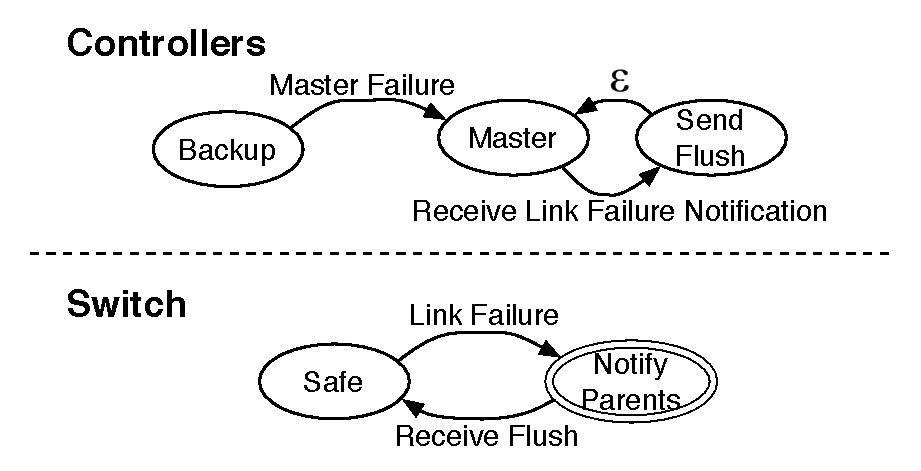
\includegraphics[width=3.25in]{../diagrams/state_machines/controller_switch.pdf}
    \caption[]{\label{fig:state_machines} Simplified state machines for the switch and
    controllers in the example Floodlight bug. Double outlined states
    represent presence of the blackhole.}
\end{figure}
}

We then consider an
internal event $i'$ observed in $replay$
equivalent (in the sense of inheriting all of its happens-before relations) to an internal
event $i$ from the original log if and only if all unmasked fields have the same value
and $i$ occurs between $i'$'s preceding and succeeding inputs in the
happens-before relation.\\[0.5ex]
%
\noindent {\bf Handling Absent Internal Events.} Some internal events from the original
log that ``happen before'' some external input
may be absent when replaying a subsequence.
For instance, if we prune a link failure,
the corresponding notification message will not arise.
\eat{
The control software's state machine (which we do not assume to know) determines whether
internal events cease to appear. Consider the simplified state machines for the switch and
controllers from the Floodlight case shown in
Figure~\ref{fig:state_machines}. If we prune the link failure input, the
master will never receive a link failure notification and
transition to and from \emph{Send Flush}.}

\eat{ % Somewhat redundant with peek()
\begin{figure}
  \footnotesize
  \begin{pseudocode}[framebox]{CausalInference}{events}
    \PROCEDURE{Replay}{subsequence}
    subsequence \GETS \CALL{Peek}{subsequence} \\
    \FOR e\textsubscript{i}\ in\ subsequence \\
      \BEGIN
      \IF e\textsubscript{i}\ is\ an\ internal\ event \\
      \AND e\textsubscript{i}\ is\ not\ marked\ absent:
      \THEN
        \BEGIN
          \Delta \GETS |e\textsubscript{i}.time - e\textsubscript{i-1}.time| + \epsilon \\
          wait\ up\ to\ \Delta\ seconds\ for\ e\textsubscript{i} \\
          \IF e\textsubscript{i}\ did\ not\ occur:
          \THEN mark\ e\textsubscript{i}\ as\ absent
        \END
      \ELSEIF e\textsubscript{i}\ is\ an\ input:
      \THEN
        \BEGIN
          \IF a\ successor\ of\ e\textsubscript{i}\ occurred: \\
          \INLINECOMMENT{waited too long}
          \THEN
            \RETURN{\CALL{Replay}{subsequence}}
          \ELSE
            inject\ e\textsubscript{i}
          \END
        \END
    \ENDPROCEDURE
  \end{pseudocode}
  \caption{{\tt Replay} is responsible for replaying subsequences of events
  chosen by delta debugging and determining
  if the bug reappears. \colin{Fix framebox width.}}
    \label{fig:replay}
\end{figure}
}

\begin{figure}
  \footnotesize
  \begin{pseudocode}[framebox]{Peek}{events}
    \PROCEDURE{Peek}{input\ subsequence}
    inferred \GETS [\ ] \\
    \FOR e\textsubscript{i}\ in\ subsequence \\
    \BEGIN
      checkpoint\ system \\
      inject\ e\textsubscript{i} \\
      \Delta \GETS |e\textsubscript{i+1}.time - e\textsubscript{i}.time| + \epsilon \\
      record\ events\ for\ \Delta\ seconds \\
      matched \GETS original\ events\ \&\ recorded\ events \\
      inferred \GETS inferred + [e\textsubscript{i}] + matched \\
      restore\ checkpoint\\
    \END \\
    \RETURN{inferred}
    \ENDPROCEDURE
  \end{pseudocode}
  \caption{{\sc Peek} determines which internal events
  from the original sequence occur for a given subsequence.
  \label{fig:peek}}
  \vskip -1.2em
\end{figure}

To avoid waiting forever we infer the presence of internal
events before we $replay$ each subsequence. Our algorithm (called {\sc Peek()}) for inferring the
presence of internal events is depicted in
Figure~\ref{fig:peek}. The algorithm injects each input, records a checkpoint\footnote{We discuss the implementation details of checkpointing
in~\cite{sts2014}.} of
the network and the control software's state, allows the system to proceed up
until the following input (plus a small time $\epsilon$), records the observed
events, and matches the
recorded events with the functionally equivalent internal events observed in
the original trace.\footnote{In the
case that, due
to non-determinism, an internal event occurs during {\sc Peek()} but does not occur
during $replay$, we time out on internal events after $\epsilon$ seconds of
their expected occurrence.}\\[0.5ex]
%
%\eat{ % Old version without peek()
%We handle this possibility by waiting for each expected internal event
%for a certain time \textepsilon. If the internal event does not occur within
%this time, we assume that it is absent and proceed. If, however, we find
%during the \textepsilon~time units we were waiting that another internal that
%happens \emph{after} our next input occurs, we know that we have waited too
%long and violated causality. In this case we need to restart the replay
%process, this time knowing which internal events in the current
%input interval are and are not going to occur before injecting the next input.
%We show our overall event scheduling algorithm
%in Figure~\ref{fig:replay}.
%}
%
\noindent {\bf Handling New Internal Events.} The last possible induced change is the occurrence of new
internal events that were not observed in the original log.
New events present multiple possibilities for where
we should inject the next input. Consider the following case:
if $i_2$ and $i_3$ are internal events observed
during $replay$ that are both in the same equivalence class as a single event $i_1$ from the
original run, we could inject the next input after $i_2$ or after $i_3$.

% TODO: figure this figure out
%\begin{wrapfigure}{c}{1.3\linewidth}
%  \centering
%  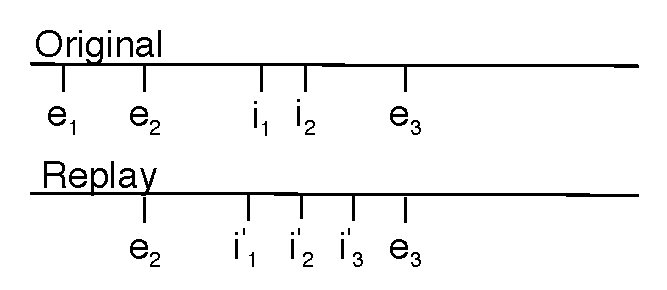
\includegraphics[width=\linewidth,height=0.8in]{../diagrams/state_machines/event_sequence.pdf}
%\end{wrapfigure}

In the general case it is always possible to construct two state machines that lead
to differing outcomes: one that only leads to the invariant violation when
we inject the next input
\emph{before} a new internal event, and another only when we inject \emph{after} a new internal
event. In other words, to be guaranteed to traverse any state transition suffix that leads
to the violation, we must recursively branch, trying both
possibilities for every new internal event. This implies an exponential worst
case number of
possibilities to be explored.

\setlength\extrarowheight{0.8pt}

\begin{table*}[ht!]
\centering
\footnotesize
\begin{tabular}{|l||l|l|r|r|r|r|l|}
  \cline{2-8}
  \multicolumn{1}{c|}{~} & \textbf{Bug Name} & \textbf{Topology} &
  \textbf{Runtime (s)} & \textbf{Input Size} & \textbf{MCS Size} &
  \textbf{MCS WI} & \textbf{MCS Helpful?}  \\\cline{2-8} \hline
  \multirow{7}{*}{\rotatebox[origin=c]{90}{\bf Newly Found}}
& Pyretic Loop & 3 switch mesh & 266.2 & 36 & 1 & 2 & Yes \\
% 20/20
% experiments/new_pyretic_loop_mcs/
% Total original inputs: 36
& POX Premature PacketIn & 4 switch mesh & 249.1 & 102 & 2 & NR & Yes \\
% 20/20
% Andi: experiments/pox_early_packetin_mcs
% Total inputs: 102
& POX In-Flight Blackhole & 2 switch mesh & 1478.9 & 27 & 11 & NR & Yes \\
% \colin{15/20 [20/20*]}
% Updated: experiments/pox_inflight_blackhole_mcs_dp_internal
& POX Migration Blackhole & 4 switch mesh & 1796.0 & 29 & 3 & NR & Yes \\
% 20/20
% Total inputs: 29
% With DP events: 117/3
% fuzz_pox_4mesh_blackhole_mcs, pox_blackhole branch of experiments repo
%& POX list removal & 2 switch mesh & 20/20 & 2 & Yes \\
%% Total inputs: 69
%% With DP events: 72/2
%% Original: config/eugene_epsilon_replay.py
%% MCS: config/eugene_epsilon_mcs.py
& NOX Discovery Loop & 4 switch mesh & 4990.9 & 150 & 18 & NR & Indirectly \\
% 18/20
% Total inputs: 150
% With DP events: 358/58
% Original: ce547fc1df3bde279b6f3dd589c909663e295f1e
% MCS: 5f49e791b0c1a611454cf0930f54aa609dd635d3
% Updated to new format: nox_mesh_4_loop_repro_verbose
& Floodlight Loop & 3 switch mesh & 27930.6 & 117 & 13 & NR & Yes \\
% 15/50
% Total inputs: 284
% zeta_final/, on floodlight branch of experiments repo
& ONOS Database Locking & 2 switch mesh & N/A & 1 & 1 & 1 & N/A \\
% onos_db_lock_mcs/
\hline
\hline
\multirow{3}{*}{\rotatebox[origin=c]{90}{\bf Known}}
& Floodlight Failover & 2 switch mesh & - & 202 & 2 & - & Yes \\
% Predates the experiment directory
& ONOS Master Election & 2 switch mesh & 2746.0 & 20 & 2 & 2 & Yes \\
% onos_id_bug_fixed_ids_file_mcs4/
& POX Load Balancer & 3 switch mesh & 2396.7 & 106 & 24 (N+1) & 26 & Yes \\
% load_balancer_fuzzer_mcs/
% Total original inputs: 106
% --------
%ONOS forgotten flows & TBD & TBD & TBD \\
\hline
\hline
\multirow{7}{*}{\rotatebox[origin=c]{90}{\bf Synthetic}}
& Delicate Timer Interleaving & 3 switch mesh & N/A & 39 & NR & NR & No \\
% experiments/snapshot_demo_synthetic_link_failure
% total original inputs: 39
& Reactive Routing Trigger & 3 switch mesh & 525.2 & 40 & 7 & 2 & Indirectly \\
% experiments/experiments/pox_broken_floyd_mcs
% total original inputs: 40
% MCS is inflated! link failure / recovery in MCS not related to triggering events.
& Overlapping Flow Entries & 2 switch mesh & 115.4  & 27 & 2 & 3 & Yes \\
% experiments/trigger_priority_mismatch_small_mcs
% total original inputs: 27
& Null Pointer & 20 switch FatTree & 157.4 & 62 & 2 & 2 & Yes \\
% experiments/experiments/pox_null_pointer_mcs
% total original inputs: 365
& Multithreaded Race Condition & 10 switch mesh & 36967.5 & 1596 & 2 & 2 & Indirectly \\
% experiments/trigger_multithreading_bug_mcs
% total original inputs: 1596
& Memory Leak & 2 switch mesh & 15022.6 & 719 & 32 (M+2) & 33 & Indirectly \\
% experiments/trigger_memory_leak3_mcs/
% total original inputs: 719
%Execution-speed race condition & 3 switch mesh & - & 9 & Yes \\
%% "floodlight" branch: experiments/floodlight_loop_2014_mcs_*
%% Total original inputs: 157
& Memory Corruption & 4 switch mesh & 145.7 & 341 & 2 & 2 & Yes \\
% syn_mem_corruption_3switch_fuzzer_mcs
% Total original inputs: 341
% ----
%Latency spike & TBD & TBD & TBD \\
%Invalid sleep value & TBD & TBD & TBD \\
%Non-deterministic TCAMs -> transient tenant isolation breach & TBD & TBD & TBD \\
%Decision based on last byte of TCP SYN & TBD & TBD & TBD \\
\hline
\end{tabular}
\caption{Overview of Case Studies. `WI' denotes `Without Interposition', and
`NR' denotes `Not Replayable'.}
\label{tab:case_studies}
\vskip -1em
\end{table*}

\setlength\extrarowheight{0pt}




Exponential search over these possibilities is not a practical option. Our heuristic
is to proceed normally if there are new internal events,
always injecting the next input when its last expected predecessor
either occurs or times out. This ensures that we always find state transition suffixes that
contain a subsequence of the (equivalent) original internal events, but leaves open the
possibility of finding divergent suffixes that lead to the invariant
violation.\\[0.5ex]
% Cut if we need space:
%This is reasonable because not even branching on new
%internal events is guaranteed to find the globally shortest fault-inducing input
%sequence:
%there may be other unknown
%paths through the state machine leading to the invariant violation that are
%completely disjoint from the original execution.
%
%\eat{
%Luckily, crucially ambiguous new internal events are not problematic for the
%control software we evaluated, as we show in \S\ref{sec:casestudies}.
%We conjecture that ambiguous new internal events are
%rare because SDN software is a control plane system,
%and is designed to quiesce quickly (\ie~take a small number of internal
%transitions after any input event, and stop at highly connected vertices).
%Concretely, SDN programs are often structured as (mostly independent) event
%handlers, meaning that pruning input events simply triggers a subset of the original
%event handlers.
%\eat{
%As an illustration, consider the state machines
%in Figure~\ref{fig:state_machines}:
%the controllers quickly converge to a single state (either ``Master'' or
%``Backup''), as do the switches (``Safe'').
%}
%}
%
\noindent {\bf Recap.} We combine these heuristics to replay each
subsequence chosen by delta debugging: we compute functional equivalency
for all internal events intercepted by our test orchestrator's
interposition layer, we invoke {\sc Peek()} to infer absent internal events,
and with these inferred causal dependencies we $replay$
the input subsequence, waiting to inject each input until each of its
(functionally equivalent) predecessors have occurred while allowing
new internal events through the interposition layer immediately.\\[0.5ex]
%
\noindent {\bf Results.} We briefly describe an evaluation of these
techniques. For a full evaluation, see~\cite{sts2014}.

We summarize the results of our evaluation in Table~\ref{tab:case_studies}.
The table contains the results of case studies we ran on
five open source SDN control platforms:
ONOS~\cite{ONOS} (Java), POX~\cite{pox} (Python), NOX~\cite{nox} (C++),
Pyretic~\cite{frenetic} (Python), and Floodlight~\cite{floodlight} (Java), and
debugged these with the help of \projectname. The case studies include seven
bugs we found with fuzz testing, as well as a demonstration of the
boundaries of where \projectname~works well and where it does not on
previously known and synthetic bugs that span a range of bug types
encountered in practice.

We note that with the exception of Delicate Timer
Interleaving and ONOS Database Locking, \projectname~was able to significantly reduce input traces.
The MCS WI column, showing the MCS sizes we produced when ignoring internal events entirely,
indicates that our techniques for interleaving
events are often crucial.
In one case however---Reactive Routing Trigger---non-determinism was particularly
acute, and \projectname's interposition on internal
events actually made minimization worse due to timeouts on
inferred internal events that did not occur after {\sc
Peek()}. In this case we found
better results by simply turning off interposition on internal events.
For all of the other case studies, either non-determinism was not problematic, or we were able to
counteract it
by replaying multiple times per subsequence and adding instrumentation.

The cases where \projectname~was most useful were those where a developer would
have started from
the end of the trace and worked backwards, but
the actual root cause lies many events in the past (as in Memory Corruption).
This requires many re-iterations through the code and logs using standard
debugging tools (\eg~source level debuggers), and
is highly tedious on human timescales. In contrast, it was easy to step
through a small event trace and manually identify the code paths responsible
for a failure.

Bugs that depend on fine-grained thread-interleaving or timers
inside of the controller are the worst-case for \projectname. This
is not surprising, as they do not directly depend on the input events from the
network, and we do not directly control the internal scheduling and timing
of the controllers. The fact that \projectname~has a difficult time reducing
these traces is itself indication to the developer that fine-grained non-determinism is at
play.


\section{Future Work}
\label{sec:future_work}
The scheduling heuristics we developed in the previous section have several
shortcomings. Most importantly, treating the software as a blackbox disallows us
from showing formal properties of the MCSes we produce. That is, we cannot
explain why our outputs are good approximations to truly minimal sequences, nor can we
explain how the heuristics helped. Second,
although we do not believe that the techniques are
specific to SDN control software, they currently pertain only to that specific
domain. Here we outline plans to address both of the these shortcomings.
At a high level, we plan to (i) start with an infeasible but provably correct
approach, and
(ii) find practical approximations to this approach, many of which will
involve leveraging empirical properties of (iii) different classes of distributed software
systems (beyond just SDN control software).

\noindent{\bf Showing Formal Properties of MCSes.} If we were to repeatedly
$replay$ a
fixed subsequence of external events $E_S$ to a blackbox distributed system,
it is possible that it would not to produce the same output on each
execution, even if we were to apply the heuristics outlined in
\S\ref{sec:past_work}. The issue is that we do not have full visibility into internal
events nor control over the internal scheduling decisions of the distributed
system. Our approach in~\cite{sts2014} was to
replay each subsequence multiple times, but this does not provide any
guarantees on the minimality of the MCSes we produce, since it's possible that
a subsequence $E_S$ that we thought did not reproduced the invariant violation
could have done so if the
distributed system had interleaved its internal events in some other way.

Suppose we want to show how close our outputs are to minimal. One approach would be to use a model checker to
{\em certify} whether each subsequence $E_S$ chosen by delta debugging does or
does not reproduce the original violation, thereby producing a provably
minimal MCS. The model checker could accomplish this
by systematically exploring all possible interleavings of internal events
given the fixed sequence of external events $E_S$.\footnote{Note that the
internal events are not fixed. That is, the schedule chosen by the model
checker affects which internal events are subsequently triggered by the software under
test.}

\noindent{\bf Working Around Impossibility.} In some cases, it is not possible for the model checker to certify a
given subsequence $E_S$. For example, suppose that the distributed system does
not terminate (or more specifically, suppose its state space is infinite
and non-recurring). In that case, model checking is not guaranteed to terminate.
Crucially, if the
model checker does not find a way to trigger the original violation in finite time,
that does not imply that the violation cannot be triggered, and we therefore lose our guarantees on minimality.

In distributed systems, non-termination means that an algorithm is not guaranteed to stop
sending messages. The formal term for this property is `non-quiescence`. In~\cite{aguilera1997heartbeat} Aguilera et al. prove that
all failure detectors---an important algorithmic component used by many distributed systems---are
non-quiescent.

As a fallback to non-quiescence, we can resort to
bounded model checking, where the model checker only explores the event
interleavings for a given subsequence $E_S$ up to a certain number of
execution steps. This approaches weakens the soundness (minimality) guarantees provided by
our approach in favor of the ability to operate on real distributed
systems implementations.

In some cases, we can also leverage the following observation to work around
non-quiescence:
given a failure detector component, it is possible to implement many other
distributed algorithms in a quiescent manner~\cite{aguilera1997heartbeat}. Building on this observation,
one might mark (non-quiescent) failure detector algorithms as `trusted-components`,
such that the model checker takes control of when the failure detector reports
failures and recoveries to the application, and systematically explores when
these failure/recovery reports are triggered in order to certify the remaining
(quiescent) components of the distributed system.

\noindent{\bf Making Certification Practical.} Although we only use the
model checker to find specific invariant violations rather than asking it to
find all invariant violations, it may nonetheless need to explore an
intractable number of event interleavings. This would make it impractical for
use on real distributed software.

We believe that we can ameliorate computational intractability by
leveraging the prior knowledge contained in the original failing test case.
That is, by making the $replay$ function stateful, we can develop heuristics that lead the
model checker to quickly find interleavings that trigger the original violation, so that
it is only forced to enumerate all interleavings for subsequence $E_S$ that do
not trigger the original violation.

As a concrete example, if we lead
the model checker to first explore interleavings that have small edit
distances from the original execution, we hypothesize that its probability of
finding the same invariant violation within the first few explored scheduled
will increase dramatically versus randomly choosing schedules to explore.
If the model checker can find violation-triggering schedules in $O(N)$ time rather than $O(2^N)$ time
(where $N$ denotes the number of events to schedule),
the asymptotic complexity of the overall minimization process can be reduced.
We will evaluate these heuristics empirically, by measuring the number of
interleavings that need to be explored for event traces where we know
MCS {\em a priori}. Often, we will develop these heuristics by examining the
behavior of specific distributed systems, as we describe next.

\noindent{\bf Applying to Other Distributed Systems.} In~\cite{sts2014} we
only applied our techniques to SDN control software. We do not however believe
that our techniques are specific to SDN. We have already begun applying our
techniques to other kinds of distributed systems, including distributed
databases and consensus protocols. One contribution of our work will be to
tailor our minimization strategies so that they
leverage the properties of those systems (e.g. atomic transactions in the
domain of distributed databases) or their empirical behavior (e.g. a tendency
to trigger violations along certain schedules) in
order to make the minimization process more practical.

% Left-behind ideas / lines of work:

% 1. exploring the "interposition tradeoff"? Iterate through the levels
% programmatically -- probably the case that different bug types necessitate
% different kinds of interposition. Also, look into modularizing model checking,
% a la JunFeng's work on demeter.

% 2. using Synoptic to generate model of the software.

% 3. Are Panda's email chains on modelling computational structure relevant?

% 4. Black-box delta debuggin on Jepsen.

% 5. Showing how to apply the techniques to production systems rather than QA
% tests.

% 6. Taint tracking / provenance

% 7. Dataflow analysis for filtering inputs. Possibly: dataflow analysis on
% network , but not controllers.

% 8. Optimizing delta debugging

% 9. Distinguishing between persistent and transient violations.

% 10. Using delta debugging to isolate differences, not just minimize whole test


\section{Timeline}
\label{sec:timeline}
Before closing, we present a timeline for completion of the proposed research:

\begin{itemize}
\item Complete: [SIGCOMM 2014] Presented work on identifying minimal sequences without making assumptions about the
language or instrumentation of the software under test~\cite{sts2014}.
\item Planned: [SOSP 2015] Work on (i) finding an infeasible but provably correct
approach, and (ii) finding practical approximations to this approach, many of which will
involve leveraging empirical properties of (iii) different classes of distributed software
systems (beyond just SDN control software).
\item Graduation: Winter 2015 / Spring 2016.
\end{itemize}


\footnotesize{\bibliographystyle{abbrv}
\bibliography{bib}
}

\end{document}
